\chapter{Tecnologías para el desarrollo. Herramientas utilizadas}
\noindent
\drop{L}a plataforma de juego propuesta, está compuesta de varios de elementos «hardware» que permiten el diseño y ejecución de un prototipo de pruebas para la ejecución del presente TFG, obteniendo un sistema que integra las características de los sistemas tangibles aplicados en el ámbito educativo en niños de corta edad.

\section{Hardware.}

Se conoce como Hardware, al conjunto de elementos físicos que trabajan conjuntamente como unidad, y que componen un sistema informático.

\subsection{Raspberry Pi 3.}

Raspberry Pi es un dispositivo hardware de placa única de bajo coste, empleado para diversas aplicaciones en proyectos de electrónica.\

Los actuales sistemas informáticos con los que un niño puede interactuar diariamente normalmente estarán bloqueados impidiendo que puedan ser utilizados creativamente como herramienta. Raspberry Pi surge como solución a este tipo de problema. Fue desarrollado por la \textbf{Raspberry Pi Fundation} en la Universidad de Cambridge (Reino Unido) con el objetivo de estimular la enseñanza de «Ciencias de la Computación» en las escuelas ~\cite{Upton}. 

\subsubsection{Datos técnicos de «Raspberry Pi 3»}

El modelo de Raspberry Pi 3 (ver Figura~\ref{fig:Propuesta1registros}) utilizado para la plataforma de juego, dispone de las siguientes características técnicas:

\begin{itemize}
\item \textbf{Procesador Broadcom BCM2837.} Este procesador es el primero que dispone de soporte de 64 bits en lugar de 32 bits, siendo significativamente mas rapido que su predecesor (\textbf{BCM2836}), el cual se encuentra en \textbf{Raspberry Pi 2}.

\item \textbf{Comunicaciones inalámbricas.} Este modelo es el primero en incorporar soporte inalámbrico, con una capacidad de conectarse a redes Wi-Fi de 2,4 GHz, al igual que a dispositivos «Bluetooth».

\item \textbf{Puertos de entrada/salida.} Dispone de una cabecera GPIO\footnote{del ingles general-purpose input/output} de 40 pines.

\item \textbf{Comunicaciones USB.} Este dispositivo cuenta con cuatro puertos USB, lo que permite conectar cualquier tipo de periféricos (teclados, ratos, memorias USB, etc...)

\item \textbf{Puerto Ethernet.} Mediante el uso de un cable Ethernet, el dispositivo puede ser conectado a una red LAN para transferencia de información.

\item \textbf{Puerto HDMI.} Este puerto sirve para conectar un dispositivo de salida, para mostrar la interfaz gráfica de usuario del dispositivo.

\item \textbf{Puerto MicroSD.} Dispone de una ranura para tarjeta «MicroSD» que es utilizada para albergar el sistema operativo.

\item \textbf{Alimentación MicroUSB.} El dispositivo es alimentando por medio de un puerto de carga tipo «MicroUSB».

Las características han sido obtenidas de \textbf{Raspberry Pi User Guide ~\cite{Upton}}

\end{itemize}

\begin{figure}[!h]
\begin{center}
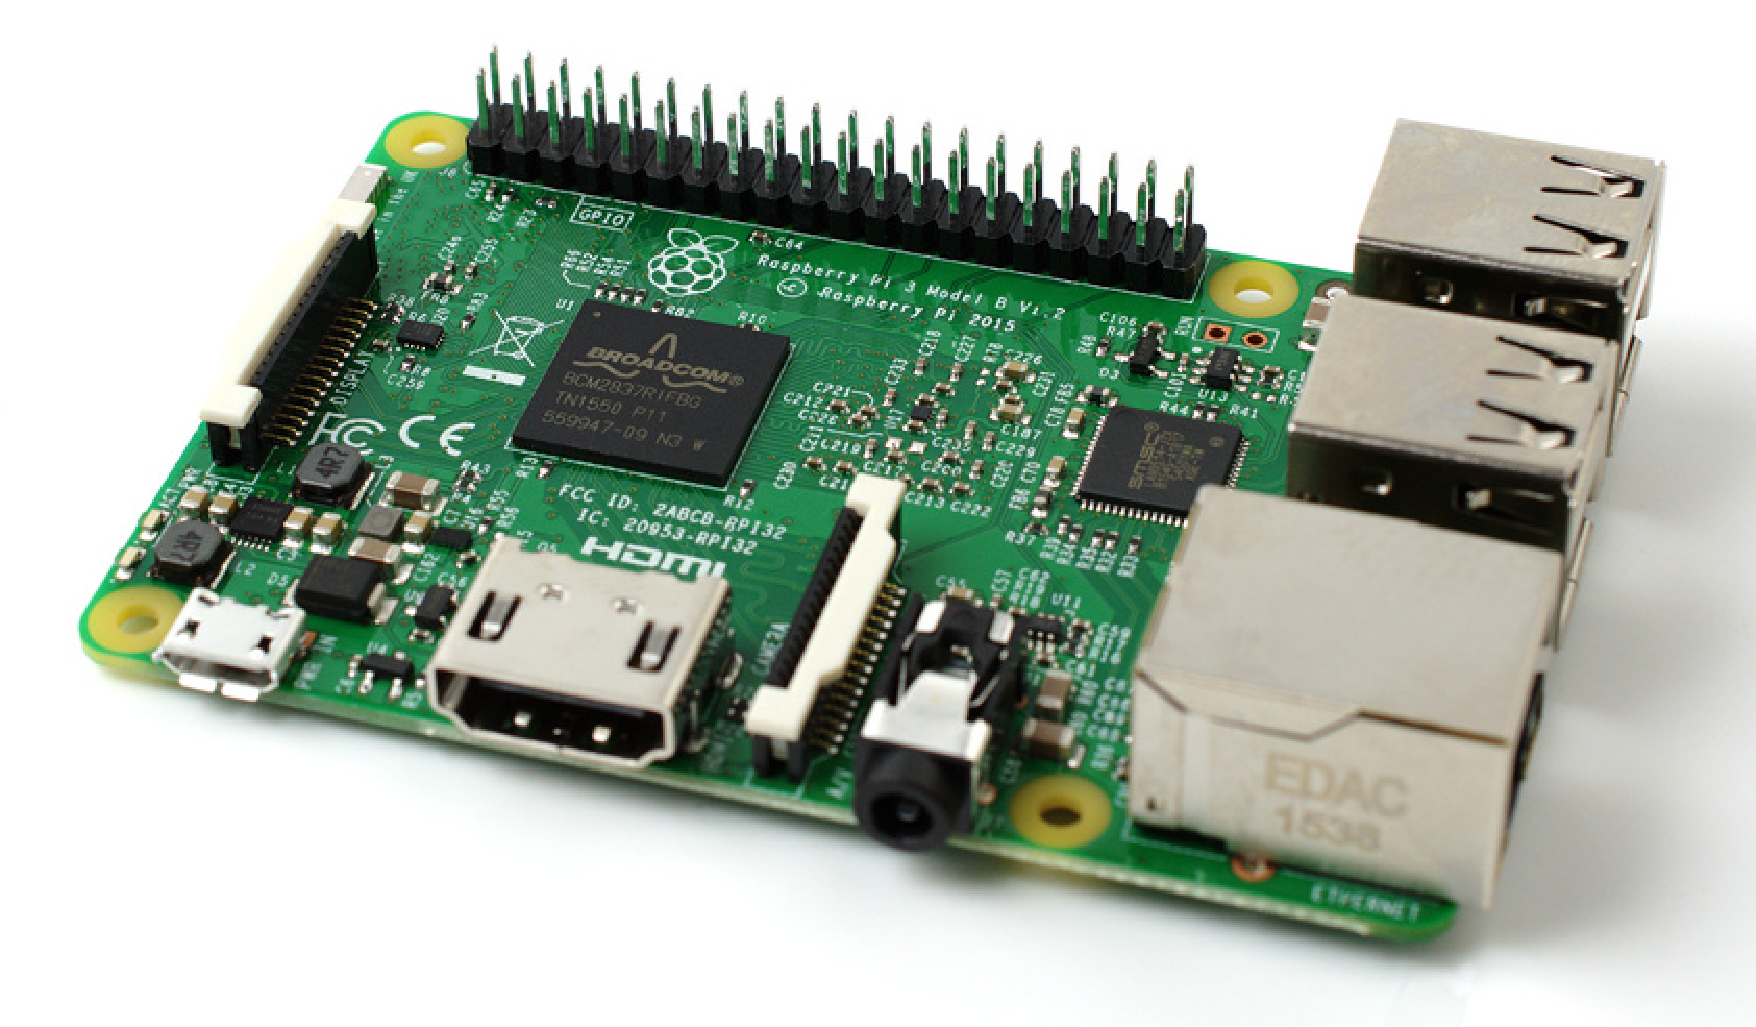
\includegraphics[width=0.7\textwidth]{Raspberry3.pdf}
\caption{Placa Raspberry Pi 3. Fuente: ~\cite{Upton}}
\label{fig:Raspberry3}
\end{center}
\end{figure}


\subsection{Interfaz entrada/salida (Pantalla multitáctil).}
La gran mayoría de los dispositivos comercialmente disponibles actualmente y que hacen uso de una pantalla, usan la tecnología de contacto capacitivo. Estas tecnologías no solo ofrecen un entorno gráfico, sino simplifican la interacción \textbf{HCI} mediante el sentido del tacto.\

La pantalla multitáctil capacitiva utilizada en la plataforma de juego, y que es incorporada al dispositivo \textbf{TUIO1}, es el modelo \textbf{7inch HDMI LCD (C)} de la compañía \textbf{Waveshare}.
\subsubsection{Datos técnicos de la pantalla de Waveshare «7inch HDMI LCD (C)»}



\subsection{Dispositivos de entrada. Sensores.}



\section{Entorno}




\section{Software para el desarrollo}

\subsection{Python.}

\subsection{Kivy.}
Kivy es una biblioteca de Python de código abierto y multiplataforma, la cual ofrece un conjunto de herramientas para el desarrollo de interfaces gráficas de usuario en aplicaciones multitouch.
Kivy está escrito en Python y Cython, basado en OpenGL ES 2, soporta varios dispositivos de entrada y tiene una extensa biblioteca de widgets. Con la misma base de código puede orientarse a Windows, OS X, Linux, Android e iOS. Todos los widgets de Kivy están construidos con soporte multitáctil~\cite{Kivy}. 

\textbf{Lenguaje Kv.}\\
A medida que una aplicación se vuelve más compleja, el lenguaje Kv (Kivy) permite crear Widgets de forma declarativa y vincular las propiedades de los Widgets entre sí. Permite realizar cambios agiles en la interfaz de usuario. Facilita una buena separación entre la lógica de la aplicación y la interfaz de usuario.

\textbf{Cargar Kv.}\\
Existen dos maneras de cargar código Kv en una aplicación:
\begin{itemize}
\item Mediante convenio de nombre:
Kivy busca un archivo Kv con el mismo nombre que la clase App (en minúsculas). Este archivo define un Widget raíz que se conectará al atributo raíz de la aplicación y se utilizará como base del árbol de Widgets de la aplicación.
\item Constructor: Se puede indicar a Kivy que cargue directamente una cadena o un archivo. Si esta cadena o archivo define un Widget raíz, será devuelto por el método:\\
\texttt{Builder.load\_file('path/to/file.kv')}.\\
\end{itemize}

\textbf{Normas de contexto.}\\
Una fuente Kv constituye una regla que se utiliza para describir el contenido de un Widget. Puede tener una regla raíz y cualquier número de reglas de clase o plantilla.
La regla raíz se declara en la clase del Widget raíz, sin ninguna sangría, seguida de : y se establecerá como el atributo raíz de la instancia de la aplicación:\\
\texttt{Widget:}\\
Una regla de clase que es declarada por el nombre de la clase de Widget entre <> y seguida por :, define como se representará de manera gráfica cualquier instancia de esa clase:\\
\texttt{<MyWidget>:}\\
Las reglas, al igual que en «Python», utilizan sangrías de cuatro espacios por nivel para la delimitación.\\
Existen tres palabras clave específicas del lenguaje Kv:
\begin{itemize}
\item App: siempre está referida a la instancia de la aplicación.
\item Root: hace referencia al widget base en la regla actual.
\item Self: siempre se refiere al widget actual.
\end{itemize}

\textbf{Sintaxis especiales.}\\
Existen dos sintaxis de carácter especial, que sirven para definir valores en el contexto Kv.\\
\texttt{\#:import name xyz\\
\#:import isdir os.path.isdir\\
\#:import np numpy}\\
es equivalente a:\\
\texttt{from xy import z as name\\
from os.path import isdir\\
import numpy as np}\\
en «Python».

Para establecer valores globales:\\
\texttt{\#:set name value}\\
Equivale a:\\
\texttt{name = value }\\
en «Python».\\
